\subsection{Where the gap to the published methods comes from}
\label{sec:gap}

\begin{figure}[t]
  \centering
  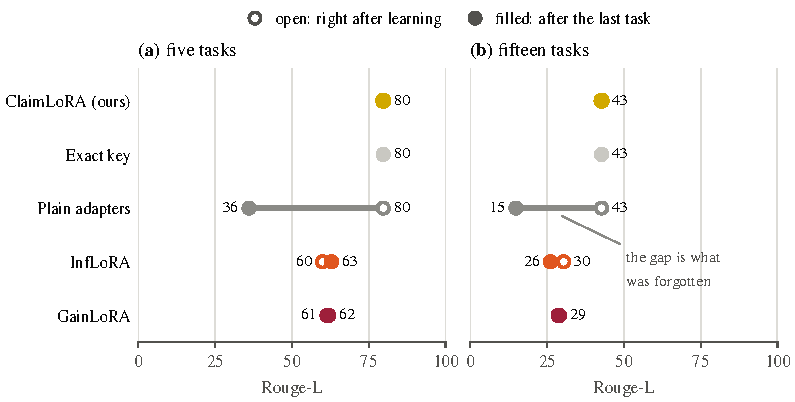
\includegraphics[width=0.9\linewidth]{figures/learn_forget}
  \caption{Learning and forgetting side by side, (a) on five tasks (mean over three seeds) and (b)
  on fifteen tasks (one seed). Open circle: average score of each task right
  after it was learned. Filled circle: average score after the last task. A gap between the two circles
  of a method is forgetting; an open circle far to the left is a lack of learning.}
  \label{fig:learnforget}
\end{figure}

Figure~\ref{fig:learnforget} separates the two things that a final score mixes.
For plain adapters the open circle is high and the filled circle is low: they learn and then forget.
For the two published methods on five tasks both circles are low and nearly equal: their forgetting scores are
near zero, but within ten epochs they have learned less. On fifteen tasks (panel b) their open circles are low
as well, and the filled circles are lower than the open ones for InfLoRA (\FifteenInfLearned{} to
\FifteenInfAP{}) and, by less, for GainLoRA (\FifteenGainLearned{} to \FifteenGainAP{}). The
certified switch has the open circle of plain adapters and no gap. On five tasks the comparison
therefore does not show that the published methods forget, and we do not claim that it does. On
fifteen tasks it shows some forgetting, and a larger lack of learning. In both, in our
set-up they had learned less by the time the next task arrived, for reasons we did not
separate (the method, the short budget, or our set-up), while the switch leaves the training of an
adapter untouched. The published results of both methods were
obtained with 100 epochs and T5-large. We could not run that setting, and the gap in learning may
well close there. Without instructions the same two methods did forget more
(Section~\ref{sec:nodefpublished}), with the same caveat on learning.
